\documentclass{article}

\RequirePackage{luatex85}
\usepackage{fontspec}
\usepackage[all]{xy}

\usepackage{fancyhdr}
\usepackage{extramarks}
\usepackage{amsthm,amsmath,amssymb,physics}
\usepackage{tikz}
\usepackage{float}
\usepackage{subcaption}
\usepackage{graphicx}
\usepackage{siunitx}
\usepackage{minted}
\usemintedstyle{vs}

% ====================
% Basic Document Settings
%

\usepackage{pgfplots}

\topmargin=-0.45in
\evensidemargin=0in
\oddsidemargin=0in
\textwidth=6.5in
\textheight=9.0in
\headsep=0.25in

\linespread{1.1}

\pagestyle{fancy}
\lhead{\hmwkAuthorName}
\chead{\hmwkClass : \hmwkTitle}
\rhead{\firstxmark}
\lfoot{\lastxmark}
\cfoot{\thepage}

\renewcommand\headrulewidth{0.4pt}
\renewcommand\footrulewidth{0.4pt}

\setlength\parindent{0pt}

%
% Create Problem Sections
%

\newcommand{\enterProblemHeader}[1]{
    \nobreak\extramarks{}{Problem \arabic{#1} continued on next page\ldots}\nobreak{}
    \nobreak\extramarks{Problem \arabic{#1} (continued)}{Problem \arabic{#1} continued on next page\ldots}\nobreak{}
}

\newcommand{\exitProblemHeader}[1]{
    \nobreak\extramarks{Problem \arabic{#1} (continued)}{Problem \arabic{#1} continued on next page\ldots}\nobreak{}
    \stepcounter{#1}
    \nobreak\extramarks{Problem \arabic{#1}}{}\nobreak{}
}

\setcounter{secnumdepth}{0}
\newcounter{partCounter}
\newcounter{homeworkProblemCounter}
\setcounter{homeworkProblemCounter}{1}
\nobreak\extramarks{Problem \arabic{homeworkProblemCounter}}{}\nobreak{}

%
% Homework Problem Environment
%
% This environment takes an optional argument. When given, it will adjust the
% problem counter. This is useful for when the problems given for your
% assignment aren't sequential. See the last 3 problems of this template for an
% example.
%
\newenvironment{homeworkProblem}[1][-1]{
    \ifnum#1>0
        \setcounter{homeworkProblemCounter}{#1}
    \fi

    \section{Problem \arabic{homeworkProblemCounter}}
    \setcounter{partCounter}{1}
    \enterProblemHeader{homeworkProblemCounter}
}{
    \exitProblemHeader{homeworkProblemCounter}
}


\newcommand{\hmwkTitle}{Homework\ \#4}
\newcommand{\hmwkDueDate}{7 May, 2020}
\newcommand{\hmwkClass}{CS364/AM792}
\newcommand{\hmwkAuthorName}{\textbf{Unathi K. Skosana}}

% Title Page

\title{
    \vspace{2in}
    \textmd{\textbf{\hmwkClass:\ \hmwkTitle}}\\
    \normalsize\vspace{0.1in}\small{Due\ on\ \hmwkDueDate\ at 17:00pm}\\
    \vspace{3in}
}

\author{\hmwkAuthorName}
\date{}

\renewcommand{\part}[1]{\textbf{\large Part \Alph{partCounter}}\stepcounter{partCounter}\\}

% Alias for the Solution section header
\newcommand{\solution}{\textbf{\large Solution}}

\begin{document}

\maketitle

\pagebreak

\begin{homeworkProblem}
  \textbf{(a)}
  \\
  \\

  The removal of outliers was done with the threshold distance of $200$ pixels. It
  is better here to use such a lenient threshold here, since the steps that
  follow involve overdetermined systems that approximate the various quantities
  of interest in the least-squares sense.

  \begin{figure}[H]
    \centering
    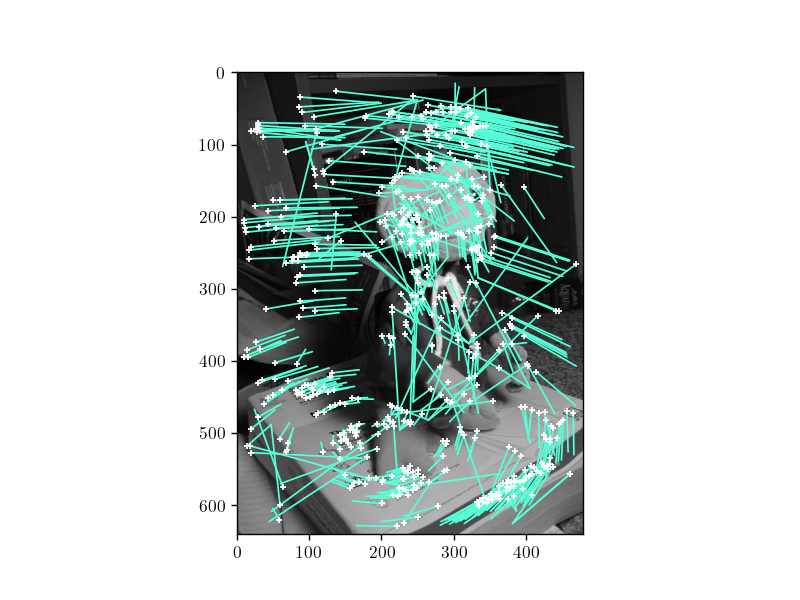
\includegraphics[width=0.8\linewidth]{images/filtered_sift_features.png}
    \caption{Filtered SIFT features}
    \label{fig:sift_feats}
  \end{figure}


  \textbf{(b)}
  \\
  \\

  Following the RANSAC procedure to estimate $F$ with a Simpson distance threshold of $1$
  pixel for $10N$ iterations where $N$ is the number of matches. The size of the
  consensus set produced was $418$ and the fundamental matrix $F$ estimated
  from the consensus set is given below

  \begin{align*}
    F = \begin{bmatrix}
      -2.48079775\mathrm{e-}6 & -1.42955448\mathrm{e-}5 & 6.24619756\mathrm{e-}3 \\
      4.57085149\mathrm{e-}6 & -1.86170164\mathrm{e-}6 & 3.59836273\mathrm{e-}2 \\
      -7.34248289\mathrm{e-}3 & -3.07400834\mathrm{e-}2 & -9.98832968\mathrm{e-}1
    \end{bmatrix}
    \label{eq:F}
  \end{align*}

  \pagebreak

  The image below shows the consensus set of matches

  \begin{figure}[H]
    \centering
    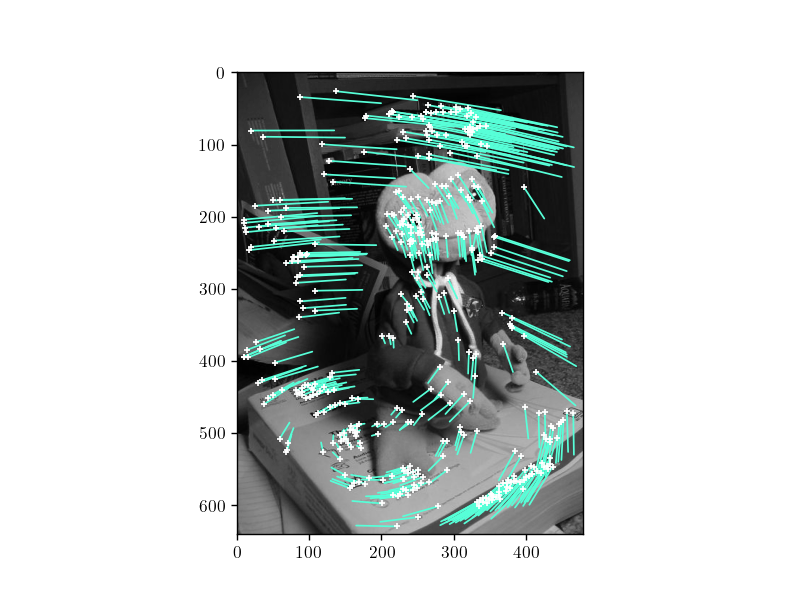
\includegraphics[width=0.8\linewidth]{images/consesus_set.png}
    \caption{Consensus set SIFT matches}
  \end{figure}

  \textbf{(c)}
  \\
  \\

  The essential matrix can be determined from the fundamental matrix and the
  calibration matrices of the cameras in a straight forward manner. Below are
  the singular values of the essential matrix in descending order.

  \begin{align*}
    \sigma_1 &= 2.50637074\mathrm{e+}1 \\
    \sigma_2 &= 2.50226239\mathrm{e+}1 \\
    \sigma_3 &= 3.11422341\mathrm{e-}15
    \label{eq:singular_values}
  \end{align*}

  and the recomputed essential matrix via the fix on handout is

  \begin{align*}
    E = \begin{bmatrix}
              1.13914812 &  6.6127527 & -0.72360584 \\
              -2.11435877 &   0.86752977 & -24.90670533 \\
              4.38710103 & 23.73844459 &   0.66624
        \end{bmatrix}
  \end{align*}

  \pagebreak

  \textbf{(d)}
  \\
  \\

  Using the calibration matrix provided for both cameras. The first camera
  matrix $P_1$ is easily determined as 

  \begin{align*}
    P_1 = \begin{bmatrix}
      677.6328 &   0.0    & 240.5   &   0.0 \\
      0.0    & 682.6328 & 320.5  &    0.0   \\
      0.0    &   0.0    &   1.0    &   0.0
    \end{bmatrix}
  \end{align*}

  A match was randomly sampled from the consensus set to triangulate its
  3-space correspondence, then this triangulated 3-space point was used to
  figure out which pair of camera matrices gives correct geometry. From this,
  $P_2$ was determined as

  \begin{align*}
    P_2 = \begin{bmatrix}
            6.15208698\mathrm{e+}2 & -9.88571941\mathrm{e+}1 &  3.58848121\mathrm{e+}2 & -5.88388075\mathrm{e+}2 \\
            4.16584571\mathrm{e+}1 & 6.76883118\mathrm{e+}2 &
            3.29850886\mathrm{e+}2 &  1.09546197\mathrm{e}+2 \\
            -1.81762243\mathrm{e-}1 &  5.49667247\mathrm{e-}3 &
            9.83327145\mathrm{e-}1 & 2.66992956\mathrm{e-}1
         \end{bmatrix}
  \end{align*}


  \textbf{(e)}
  \\
  \\
  Using the camera matrices determined above, we can triangulate all the matches
  in consensus set to produce a 3D reconstruction of the observed scene. Points
  with a $z$ coordinate further than $9$ were removed from the
  reconstruction. These points can be inaccurate due to a number of reasons i.e
  errors/noise match identification but the perhaps the most relevant here is
  the following: If a point in 3-space is very far away from the camera centres
  then the angle between the rays from the two camera centres pointing towards the point
  be quite narrow. In such a scenario the two rays will almost appear parallel
  (no intersection) and the SVD will have no exact solution for
  $A\mathbf{X} = \mathbf{0}$, thus produce an error-prone least-squares solution.

  \begin{figure}[H]
      \raggedright
      \begin{subfigure}{0.49\textwidth}
          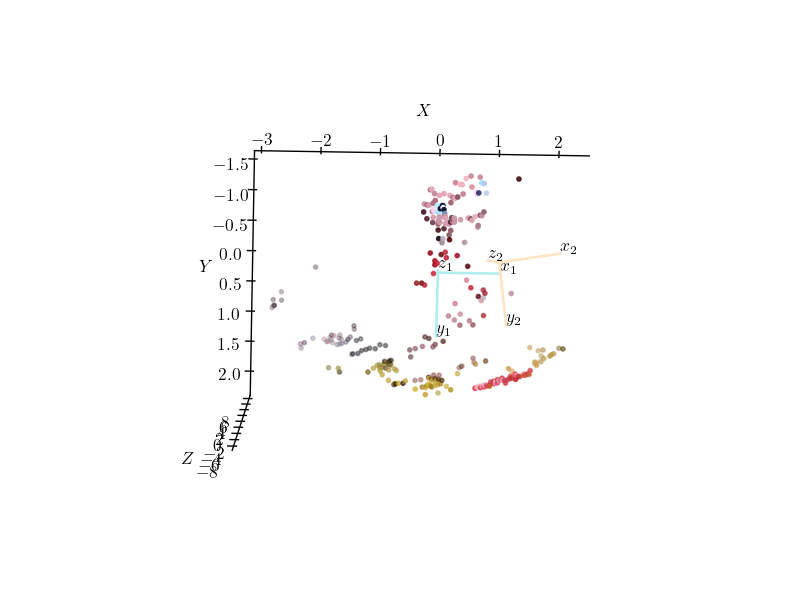
\includegraphics[width=1.3\linewidth]{images/ang_1.png}
      \end{subfigure}
      \begin{subfigure}{0.49\textwidth}
          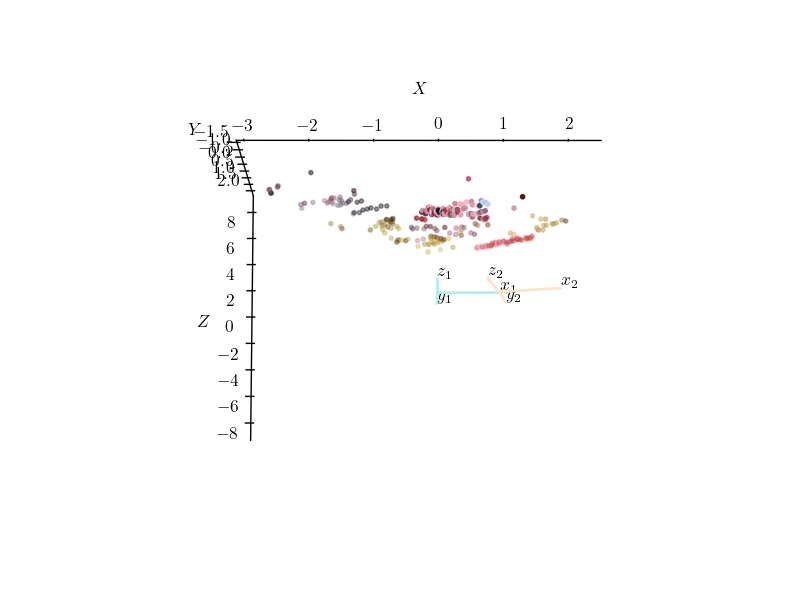
\includegraphics[width=1.3\linewidth]{images/ang_2.png}
      \end{subfigure}
  \end{figure}
  \begin{figure}[H]
      \raggedright
      \begin{subfigure}{0.49\textwidth}
          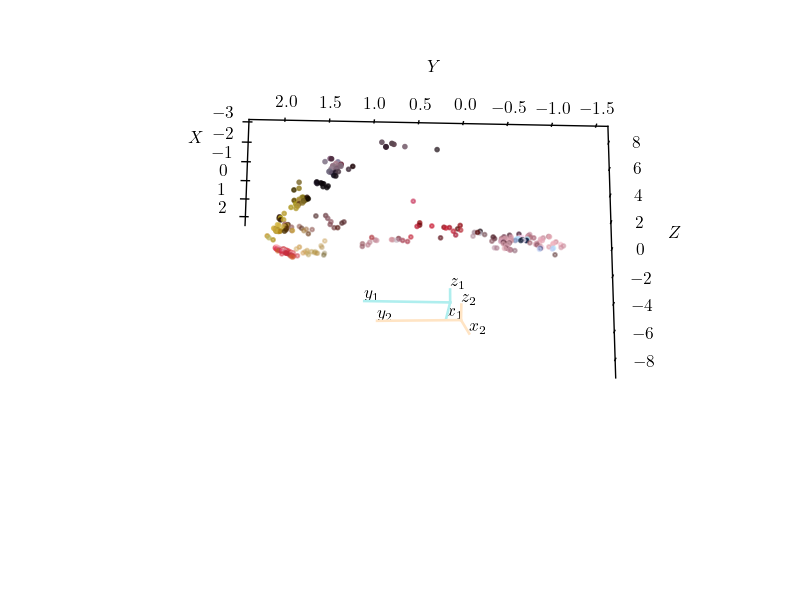
\includegraphics[width=1.3\linewidth]{images/ang_3.png}
      \end{subfigure}
      \begin{subfigure}{0.49\textwidth}
          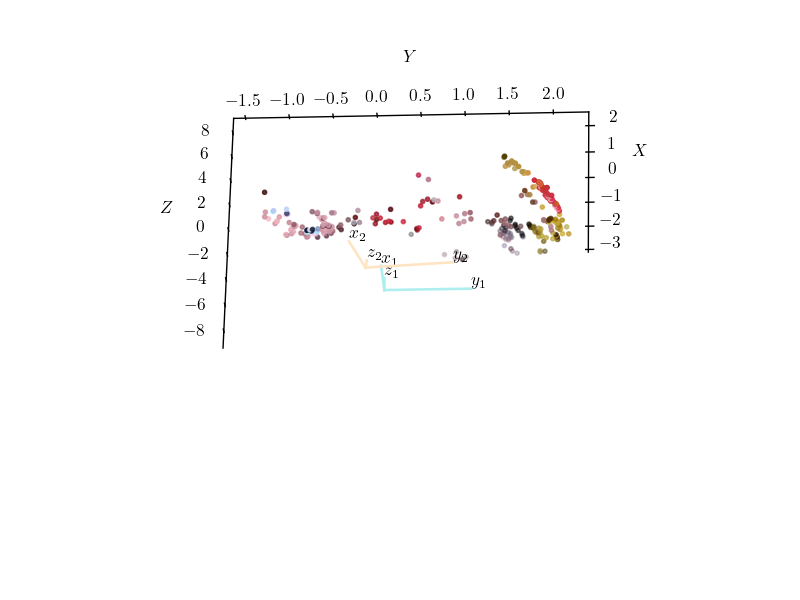
\includegraphics[width=1.3\linewidth]{./images/ang_4.png}
      \end{subfigure}
      \begin{subfigure}{0.49\textwidth}
          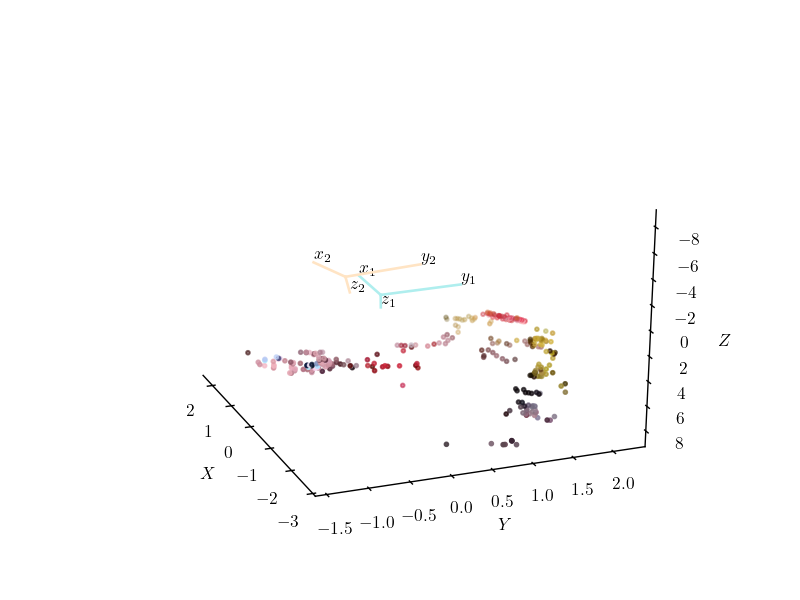
\includegraphics[width=1.3\linewidth]{./images/ang_5.png}
      \end{subfigure}
      \begin{subfigure}{0.49\textwidth}
          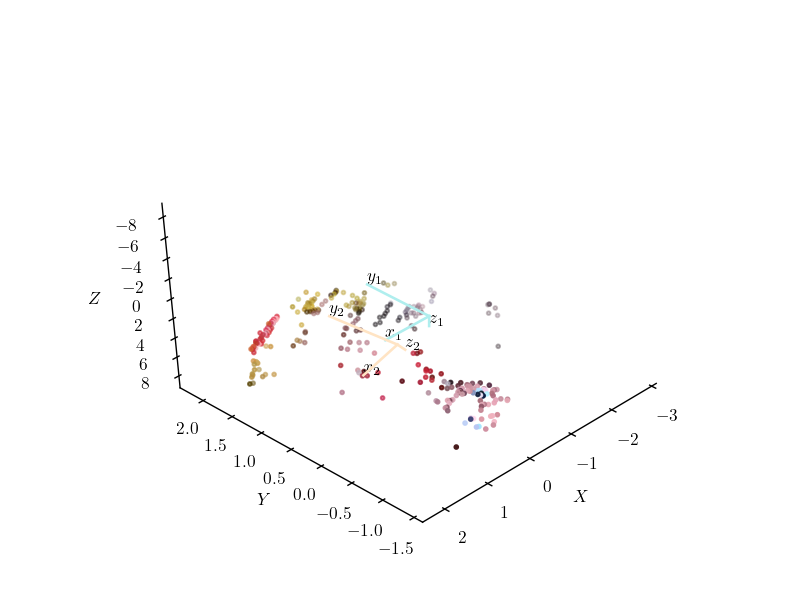
\includegraphics[width=1.3\linewidth]{./images/ang_6.png}
      \end{subfigure}
      \caption{Different views of a figure that slightly resembles ET}
    \end{figure}
\end{homeworkProblem}

\pagebreak

\begin{homeworkProblem}
  \textbf{(a)}
  \\
  \\

  Using the method already described to construct the transformation matrices
  $T_1,T_2$

  \begin{align}
    T_1 = \begin{bmatrix}
      1.01254555\mathrm{e+}0 & -1.81277806\mathrm{e-}1 & -9.53879428\mathrm{e+}0\\
      2.22458298\mathrm{e-}1 & 9.76306317\mathrm{e-}1 & -4.73204094\mathrm{e+}1 \\
      1.36222826\mathrm{e-}4 & -2.43882116\mathrm{e-}5 & 9.70646051\mathrm{e-}1
  \end{bmatrix} \\
    T_2 = \begin{bmatrix}
      1.05843644\mathrm{e+}0 & -2.66125883\mathrm{e-}2 & -1.98319624\mathrm{e+}2\\
      1.55922518\mathrm{e-}1 & 1.00836582\mathrm{e+}0 & -7.13240170\mathrm{e+}1\\
      4.01122752\mathrm{e-}4 & 2.84646210\mathrm{e-}5 & 8.56560707\mathrm{e-}1
    \end{bmatrix}
  \end{align}

  we can warp the original images to produce

  \begin{figure}[H]
      \centering
      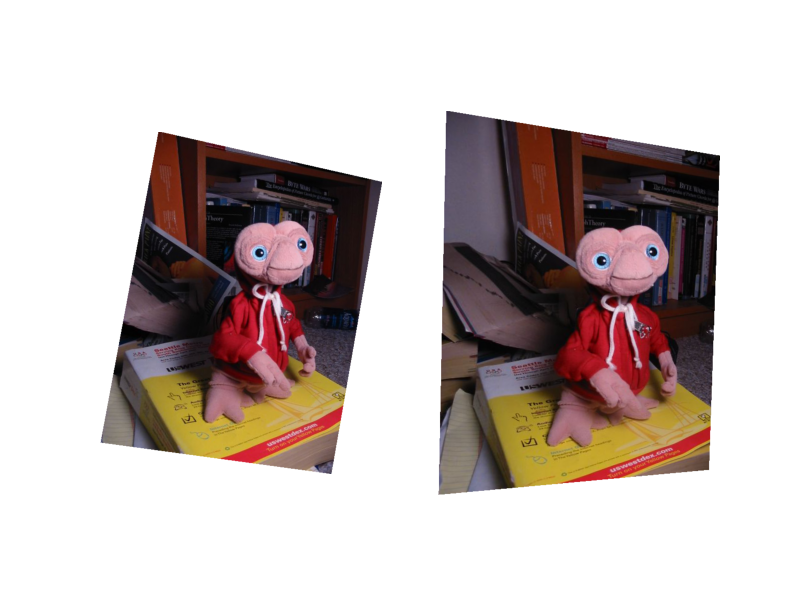
\includegraphics[width=1.0\linewidth]{images/warped_ets.png}
      \caption{Warped ETs.}
  \end{figure}

  \textbf{(b)}
  \\
  \\

  To construct epipolar lines we have to follow the same procedure as in
  assignment 3 with the newly constructed $P'_1,P'_2$

  \begin{align}
    P'_1 &= K_nR_n [\mathbb{I} | -\tilde{\mathbf{C}}_1]\\
    P'_2 &= K_nR_n [\mathbb{I} | -\tilde{\mathbf{C}}_2]
  \end{align}

  The new fundamental matrix of the warped images is

  \begin{align}
    F' = \begin{bmatrix}
      -2.46748640\mathrm{e-}6 & -1.43590530\mathrm{e-}5 & 6.19579186\mathrm{e-}3\\
      4.73499398\mathrm{e-}6 & -1.96973184\mathrm{e-}6 & 3.55413979\mathrm{e-}2\\
      -7.25952489\mathrm{e-}3 & -3.02770122\mathrm{e-}2 & -9.98863866\mathrm{e-}1
    \end{bmatrix}
  \end{align}

  From this we can thus produce the epipolar lines in the usual way with a minor
  modification of offsetting the calculated $y$ of epipolar lines by
  $\mathrm{miny}$ used in from apply\_homography. The reason why the top-left corner
  of a rectified image may no longer coincide with the origin of the image coordinate system
  is that the homographies obtained may translation components (first two entries of third
  column are non zero) while the cameras retain their orientations
  in the world coordinate system and positions.

  \begin{figure}[H]
    \centering
    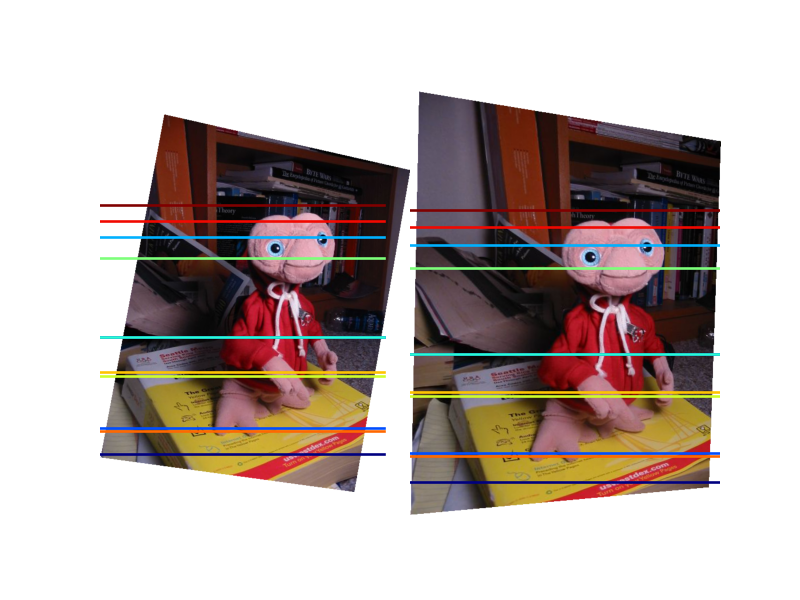
\includegraphics[width=1.0\linewidth]{images/epipolar_lines.png}
    \caption{Epipolar lines}
  \end{figure}

\end{homeworkProblem}


\end{document}
